\chapter{Wykład XIII}

\section{Pierścień noetherowski.}

\begin{definition}[Pierścień noetherowski.]
	Pierścień $R$ jest \textbf{noetherowski}, gdy każdy ideał $\mathcal{I}\unlhd R$ jest \textbf{skończenie generowany}, czyli
	\[
	\left(\exists a_1,a_2,\ldots, a_{n} \in \mathcal{I} \right)\left( \mathcal{I} = \left( a_1,a_2,\ldots,a_{n}  \right)  \right)  
	.\] 
\end{definition} 
\begin{theorem}[Nastęujące warunki są równoważne.]
	\begin{enumerate}[label=\arabic*)]
		\item Pierścień $R$ jest noetherowski.
		\item $\left(\forall \mathcal{I}_{1}\subseteq \mathcal{I}_{2} \subseteq \ldots \text{ ideały w } R \right)\left(\exists n \right)\left( \mathcal{I}_{n} = \mathcal{I}_{n-1} = \ldots  \right) \text{ (stabilizuje się ???)}  $ 
		\item Każda niepusta rodzina ideałów w $R$ ma element maksymalny
	\end{enumerate}
\end{theorem} 
\begin{proof}
	TODO
\end{proof} 
\begin{eg}
	Niech $R$ będzie PID. Wtedy $R$ jest też noetherowski.
\end{eg} 
\begin{remark}
	Jeśli \[
	R_1\underset{\scriptscriptstyle\text{podp}}{\subseteq} R_2\underset{\scriptscriptstyle\text{podp}}{\subseteq} \ldots
	,\] 
	to \[
	\bigcup_{i=1} R_{i}
	.\] 
	jest pierścieniem z sumą (teoriomnogościową) działań $+_{\scriptscriptstyle R_{i}}$ oraz $\cdot _{\scriptscriptstyle R_{i}}$.
	Definiujemy
	\[
	\underbrace{R\left[ X_1,X_2,\ldots \right] }_{\text{pierścień wielomianów zmiennych }X_1, X_2,\ldots}:= \bigcup_{i=1}^{\infty}R\left( X_1, X_2,\ldots \right) 
	.\] 
	$R\left[ X_1,X_2,\ldots \right] $ nie jest noetherowski, bo ciąg ideałów
	\[
		\left( X_1 \right) \varsubsetneq \left( X_1,X_2 \right) \varsubsetneq \left( X_1,X_2,X_3 \right) \varsubsetneq \ldots
	.\] 
	Wiemy na przykład, że $\mathbb{Z} $ jest PID oraz $\mathbb{Z} \left[ \mathbb{Z}  \right] $ nie jest PID, ale mamy twierdzenie Hilberta o bazie.
\end{remark} 
\begin{theorem}[Hilberta o bazie.]
	Załóżmy, że pierścień $R$ jest noetherowski,  wtedy $R\left[ X \right] $ jest noetherowski.
\end{theorem} 
\begin{proof}
	TODO
\end{proof} 
\begin{corollary}
	Mamy:
	\begin{enumerate}[label=\arabic*)]
		\item $R$ jest noetherowski $\implies R\left[ X_1,\ldots,X_{n}  \right] $ jest noetherowski.
		\item $K$ jest ciałem $\implies K\left[ X_1,\ldots,X_{n}  \right] $ jest noetherowski.
	\end{enumerate}
\end{corollary}
\begin{theorem}[Bez dowodu]
	$R$ jest noetherowski $\implies R\left[ \left| X \right|  \right] $ jest noetherowski.
\end{theorem} 
\begin{definition}
	Niech $R\underset{\scriptscriptstyle\text{podp}}{\subseteq} S$ oraz $a_1,\ldots,a_{n} \in S$. 

	Wtedy $R\left[ a_1,\ldots,a_{n}  \right] $ to najmniejszy podpierścień $S$ zawierający $R\cup \{a_1,a_2,\ldots, a_{n} \} $.
\end{definition} 
\begin{remark}
	\[
	R\left[ a_1,\ldots,a_{n}  \right] = \{f\underbrace{(a_1,\ldots,a_{n})}_{\text{ewaluacja}}: f\in R\left[ X_1,\ldots,X_{n}  \right] \} 
	.\] 
	Zatem $R\left[ a_1,\ldots,a_{n}  \right] $ jest obrazem homomorfizmu ewaluacji:
	\[
	\text{ev}_{\left( a_1,\ldots,a_{n}  \right) }: R\left[ X_1,\ldots,X_{n}  \right] \to S
	.\] 
\end{remark}
\begin{definition}
	Niech $K\underset{\scriptscriptstyle\text{podc}}{\subseteq} L$ oraz $a_1,\ldots,a_{n} \in L$.
	Wtedy
	\[
	K\left( a_1,\ldots,a_{n}  \right) \overset{\Def}{=} \text{ najmniejsze podciało $L$ zawierające } K\cup \{a_1,\ldots,a_{n} \} 
	.\] 
\end{definition} 
\begin{remark}
	Akurat okazało się, że
	\[
	\mathbb{Q} \left[ \sqrt{2}  \right] = \{a + b\sqrt{2} : a,b \in \mathbb{Q} \} = \mathbb{Q} \left( \sqrt{2}  \right) 
	.\] 
	Z drugiej strony \[
	\mathbb{Q} \left[ e \right] \neq \mathbb{Q} \left( e \right) \text{ (przestępność liczby $e$ )}
	.\] 
\end{remark}
\begin{theorem}
	Mamy

	\begin{enumerate}[label=\arabic*)]
		\item Niech $\varphi : R \to S $ będzie epimorfizmem pierścieni. Wtedy 
			 \[
			R\text{ jest noetherowski }\implies S\text{ noetherowski}
			.\] 
		\item $S = R\left[ a_1,a_2,\ldots,a_{n}  \right] \land R \text{ jest noetherowski} \implies S \text{noetherowski}$.
	\end{enumerate}
\end{theorem} 
\begin{proof}
	TODO
\end{proof} 
\begin{corollary}

	Mamy
	\[
	\left(\forall \alpha_1, \alpha_2,\ldots,\alpha_{n} \in \mathbb{C}  \right)\left( \mathbb{Z} \left[ \alpha_1,\alpha_2,\ldots,\alpha_{n}  \right] \text{ jest noetherowski} \right)  
	.\] 
\end{corollary}
\section{Ideały pierwsze i maksymalne.}
Chcemy uogólnić pojęcie liczby pierwszej na ideały.

Niech $n\in \N_{>1}$. Wtedy następujące warunki są równoważne:
\begin{enumerate}[label=\arabic*)]
	\item $n$ jest liczbą pierwszą.
	\item $\left(\forall a,b \in \mathbb{Z}  \right)\left( n\mid ab \implies n\mid a \lor n\mid b \right)  $.
	\item $\left(\forall a,b \in \mathbb{Z}  \right)\left( ab \in \left( n \right) \implies a\in \left( n \right) \lor b \in \left( n \right)  \right)  $.
\end{enumerate}
\textbf{Warunek 3) można przenieść na ideały.}

Niech $R$ będzie pierścieniem oraz $\mathcal{I}\unlhd R$.
\begin{definition}[Ideał pierwszy.]
	$\mathcal{I}$ jest \textbf{ideałem pierwszym}, gdy:
	\begin{enumerate}[label=\arabic*)]
		\item $\mathcal{I}\neq R$ (warunek ten odpowiada warunkowi $n\neq 1$).
		\item $\left(\forall a,b \in R \right)\left( ab \in \mathcal{I}\implies a\in \mathcal{I} \lor b \in \mathcal{I} \right)  $.
	\end{enumerate}
\end{definition} 
\begin{theorem} 
	$\mathcal{I}$ jest pierwszy $\iff \mfaktor{R}{\mathcal{I}} $ jest dziedziną.
\end{theorem} 
\begin{proof}
	TODO
\end{proof} 
\begin{corollary}
	\[
	R \text{ jest dziedziną }\iff \{\mathbf{0}\} \text{ jest ideałem pierwszym }R
	.\] 
	Bo $\mfaktor{R}{\{\mathbf{0}\} } \cong R$
\end{corollary}
\noindent \textbf{Przykłady:}
\begin{enumerate}[label=\arabic*)]
	\item Niech $n\in \mathbb{Z} $. Wtedy $\mfaktor{\mathbb{Z} }{\left( n \right) } \cong \mathbb{Z} _{n} $ ($\mathbb{Z} _{0}:= \mathbb{Z} $ ).

	Zatem $\left( n \right) $ nie jest ideałem pierwszym \[\overset{\text{twierdzenie}}{\iff } \mathbb{Z} _{n} \text{ jest dziedziną } \iff n=0 \text{ lub } n = \pm\text{liczba pierwsza}.\]
	\item \[
	\mfaktor{R\left[ X \right] }{\left( X \right) }  \cong R \text{ (używając ev$_{0}$ i zasadniczego twierdzenia homomorfizmu pierścieni)}
	.\]  
	Stąd jeżeli $R$ jest dziedziną, to $\left( X \right) $ jest ideałem pierwszym.

	Podobnie, ideał $\left( X_1,\ldots,X_{n}  \right) $ jest pierwszy w $R\left[ X_1,\ldots,X_{n}  \right] $, gdy $R$ jest dziedziną. 
\end{enumerate}
\begin{definition}
	Dla $\mathcal{I},\mathcal{J} \unlhd R$ definiujemy
	\[
	\mathcal{I} + \mathcal{J} := \{a + b : a\in \mathcal{I}\text{ oraz } b \in  \mathcal{J}\} 
	.\] 
\begin{remark}
	$\mathcal{I}+ \mathcal{J} = \left( \mathcal{I}\cup \mathcal{J} \right) $ to ideał.
\end{remark} 
\end{definition} 
\begin{definition}
	Ideał $\mathcal{I}\unlhd R$ nazywamy \textbf{ideałem maksymalnym}, gdy
	\begin{enumerate}[label=\arabic*)]
		\item $\mathcal{I}\neq R$.
		\item $\left(\forall \mathcal{J}\unlhd R \right)\left( \mathcal{I} \varsubsetneq \mathcal{J} \implies \mathcal{J} = R\right)  $
	\end{enumerate}
\end{definition} 
Poniższe twierdzenie umożliwia nam konstrukcję wielu ciał.
\begin{theorem}
	Ideał jest maksymalny wtedy i tylko wtedy, kiedy $\mfaktor{R}{\mathcal{I}} $ jest ciałem.
\end{theorem} 
\begin{proof}
	TODO
\end{proof} 

 \begin{corollary}
       $\mathcal{I}$ jest maksymalny $\implies \mathcal{I}$ jest pierwszy. 
 \end{corollary}
 \begin{proof}
 	Szkic
	\[
	\mathcal{I}\text{ maksymalny }\implies \mfaktor{R}{\mathcal{I}} \text{jest ciałem }\implies \mfaktor{R}{\mathcal{I}} \text{ jest dziedziną } \implies\mathcal{I} \text{jest pierwszy}
	.\] 
 \end{proof}
 \noindent \textbf{Przykłady:}
 \begin{enumerate}[label=\arabic*)]
	 \item $\{\mathbf{0}\} $ ideał maksymalny w $R \iff R $ jest ciałem.
	 \item $\{\mathbf{0}\} $ nie jest ideałem maksymalnym w $\mathbb{Z} $, czyli $\mathcal{I}$ maksymalny $\not\impliedby \mathcal{I}$ pierwszy.
	 \item Niech $ n\in \mathbb{Z} $. Wtedy $\left( n \right) $ jest maksymalny $\iff$
		 \[
		 \iff \mathbb{Z} _{\left| n \right| } \text{ jest ciałem } \iff n = \pm \text{liczba pierwsza}
		 .\] 
 \end{enumerate}
\begin{corollary}
     Tutaj jest użyty termin UFD, pomimo, iż nie został on wprowadzony. Czyli ten fragment jest chyba ,,zagubiony''.
     \begin{enumerate}[label=\arabic*)]
     	\item Załóżmy, że $R$ jest noetherowski oraz $\left(\forall a\in R \right)\left( a\text{ jest nierozkładalny}\implies a \text{ jest pierwsza} \right)  \implies R \text{ jest UFD}$ 
	\item z (1) PID $\implies$ UFD (???)
	\item z (2) np $K\left[ X \right] $ jest UFD oraz $\mathbb{Z} \left[ i \right] $ jest UFD
     \end{enumerate}
\end{corollary}
\begin{theorem}
	Niech $\mathcal{I}\unlhd R.$ Wtedy $\mathcal{I}$ można rozszerzyć do ideału maksymalnego.
\end{theorem} 
\begin{proof}
	TODO
\end{proof} 
\begin{remark}
	W $\mathbb{Z} $ każdy niezerowy ideał pierwszy jet maksymalny. To jest ogólnie zawsze w PID.
\end{remark} 
\begin{theorem}
	Niech $R$ będzie PID oraz $\mathcal{I}\unlhd R$ i $\mathcal{I}\neq \{\mathbf{0}\} $.
	\[
	\mathcal{I} \text{ jest pierwszy }\implies \mathcal{I} \text{ jest maksymalny}
	.\] 
\end{theorem} 
\begin{proof}
	TODO
\end{proof} 
\section{Rozkład na czynniki.}
\begin{context}

	Zakładamy teraz do odwołania, że $R$ jest dziedziną.
\end{context}
Weźmy $a\in R$, takie że $a\neq \mathbf{0}$ oraz $a\not\in R^{\ast} $.
\begin{definition}
	Definiujemy;

	\begin{enumerate}[label=\arabic*)]
		\item $a$ jest \textbf{pierwszy}, gdy 
			\[
			\left(\forall b,c \in R \right) \left( a\mid bc \implies a\mid b \lor a\mid c \right) 
			.\] 
		\item $a$ jest \textbf{nierozkładalny}, gdy 
			\[
			\left(\forall b,c \in R \right)\left( a = bc \implies b \in Rs^{\ast} \lor c \in R^{\ast}  \right)  
			.\] 
			Czyli mamy tylko \textbf{trywialne} rozkłady $a$ na iloczyn dwóch elementów, czyli rozkłady postaci
			\[
			a = \underbrace{\left( a\varepsilon ^{-1} \right) }_{b} \underbrace{\left( \varepsilon  \right) }_{c} 
			.\] 
		\item $a$ jest \textbf{nierozkładalny}, gdy nie zachodzi warunek 2)
	\end{enumerate}
\end{definition} 
\begin{remark}
	Niech $a \le R\setminus \{\mathbf{0}\} $. Wtedy
	\begin{enumerate}[label=\arabic*)]
		\item $a$ jest pierwszy $\iff $ ideał $\left( a \right) $ jest pierwszy.
		\item Następujące warunki są równoważne ($a \not\in R^{\ast} $):
			\begin{enumerate}[label=\roman*)]
				\item $a$ jest nierozkładalny,
				\item $a$ nie jest iloczynem dwóch elementów nierozkładalnych,
				\item $\left(\forall b\in R \right)\left( b\mid a \iff a\sim b \lor b \in R^{\ast}  \right)  $
			\end{enumerate}
	\end{enumerate}
\end{remark} 
\begin{proof}
	TODO
\end{proof} 
\begin{theorem}
	Niech $a\in R$, $a\neq \mathbf{0}$ oraz $a \not\in R^{\ast} $. Wtedy:
	\begin{enumerate}[label=\arabic*)]
		\item $a$ jest pierwszy $\implies a$ jest nierozkładalny
		\item $R$ jest PID oraz $a$ nierozkładalny $\implies a$ jest pierwszy.
	\end{enumerate}
\end{theorem} 
\begin{proof}
	TODO
\end{proof} 
\begin{eg}
	\begin{enumerate}[label=\arabic*)]
		\item $R = \mathbb{Z} $, $n\neq 0,1,-1$ $\left( \mathbb{Z} ^{\ast} = \{-1,1\}  \right) $
			 \[
			 n\text{ jest pierwszy } \overset{\iff}{\mathbb{Z} \text{jest PID}} \iff n \text{ jest nierozkładalny } \iff n = \pm p\text{, p liczba pierwsza}
			 .\] 
		 \item $K$ jest ciałem, $R = K\left[ X \right] $ jest PID, $f\in R\setminus K$ $\left( R^{\ast}  = K^{\ast} = K\setminus \{\mathbf{0}\}  \right) $ 
\[
f\text{ nierozkładalny }\iff f \text{ wielomian nierozkładalny w R } \iff R \text{ jest PID}
.\] 
\[
f \text{ jest pierwszy w } R \iff  \left( f \right) \text{ jest ideałem pierwszym w } R \iff \left( f \right) jest ideałem w R \iff \mfaktor{K\left[ X \right] }{\left( f \right) } \text{ jest ciałem}
.\] 
W ten sposób można skonstruować wiele ciał, np \[
	\mathbb{F} _{4} := \mfaktor{\mathbb{Z} \left[ X \right] }{\left( x^2+x+1 \right) } \text{ jest ciałem 4-element owym}
.\] 
\item $R = \mathbb{Z} \left[ \sqrt{-5}  \right] $. Rozważmy $v: \mathbb{Z} \left[ \sqrt{-5}  \right] \to \mathbb{Z} $, dane wzorem 
	\[
	v\left( n+ m\sqrt{-5}  \right) := n^2 - 5m^2 \in \N
	.\]

	W ogólności $v\left( \alpha \beta  \right) = v\left( \alpha  \right) v\left( \beta  \right) $ oraz 
	 \[
	\alpha \in \mathbb{Z} \left[ \sqrt{-5}  \right] ^{\ast} \iff v\left( \alpha  \right) = \pm \mathbf{1}
	.\] 
	\end{enumerate}
\end{eg} 
Udowodnimy, że $2\in \mathbb{Z} \left[ \sqrt{-5}  \right] $ jest nierozkładalny, ale nie jest pierwszy (w pierścieniu $\mathbb{Z} \left[ \sqrt{-5}  \right] $ ).

\begin{enumerate}[label=\arabic*)]
	\item \textbf{2 nie jest nierozkładalna w } $\mathbb{Z} \left[ \sqrt{-5}  \right] $.

		Niech $\alpha , \beta \in \mathbb{Z} \left[ \sqrt{-5}  \right],$ takie że $2 = \alpha \cdot \beta $.
		Wedy
		$v\left( \alpha  \right) v\left( \beta  \right) = v\left( \alpha \beta  \right) = v\left( 2 \right) = 4$ 

		Ale 
		\[
		\left(\forall n,m \in \mathbb{Z}  \right)\left( n^2 + 5m^2 \neq 2 \right)  
		.\] 
		Stąd $v\left( \alpha  \right) = 1$ lub $v\left( \beta  \right) = 1 \implies \alpha \in \mathbb{Z} \left[ \sqrt{-5}  \right]^{\ast} \text{ lub } \beta \in \mathbb{Z} \left[ \sqrt{-5}  \right] ^{\ast} $
	\item \textbf{2 nie jest pierwsza} 
		\[
		3\cdot 2 = 6 = \left( 1 + \sqrt{-5}  \right)\left( 1-\sqrt{5}  \right) \implies 2 \mid \left( 1 + \sqrt{-5}  \right) \left( 1-\sqrt{-5}  \right) 
		.\] 
		Ale $v\left( 2 \right)  = 4 $ i $v\left( 1\pm \sqrt{-5}  \right) = 6$. Stąd $2 \not\mid \left( 1\pm \sqrt{-5}  \right) $ w $\mathbb{Z} \sqrt{-5} $ bo $4 \not\mid 6$ w $\N$.
\end{enumerate}
\begin{remark}
	\begin{enumerate}[label=\arabic*)]
		\item w szczególności $\mathbb{Z} \left[ \sqrt{-5}  \right] $ nie jest PID ($\implies$ nie jest euklidesowa)
		\item liczba pierwsza $p \in \mathbb{Z} $ może stać się elementem rozkładalnym w większym pierścieniu, np. 
			\[
			3 = \left( 1+\sqrt{-2}  \right) \left( 1 - \sqrt{-2}  \right) \text{ w } \mathbb{Z} \left[ \sqrt{-2}  \right] \text{ ale } 1\pm \sqrt{-2} \not\in \mathbb{Z} \left[ \sqrt{-2}  \right] ^{\ast} 
			.\] 
		\item Początki algebraicznej teorii liczb. W $\mathbb{Z} \left[ \sqrt{-5}  \right] $ mamy dwa różne rozkłady 6:
			\[
			2\cdot 3 = 6 = \left( 1+ \sqrt{-5}  \right) \left( 1-\sqrt{-5}  \right) 
			.\] 
			Co to znaczy, że są one różne?
	\end{enumerate}
\end{remark} 
\section{UFD}
Załóżmy, że $R$ jest dziedziną.

\begin{definition}[UFD]
	$R$ jest UFD (dziedziną z jednoznaczności rozkładu?), gdy 
	\begin{enumerate}[label=\arabic*)]
		\item $\left(\forall a\in R\setminus R^{\ast} \cup \{\mathbf{0}\} \right)\left(\exists \underbrace{a_1,a_2,\ldots,a_{n} \in R}_{\text{nierozkładalne}} \right) \left( a = a_1\cdot a_2\cdot \ldots \cdot a_{n} \right)   $ 
		\item $\left(\forall \underbrace{b_1,\ldots,b_{k},c_1,\ldots,c_{l}}_{\text{nierozkładalne}}  \right) \left( b_1\cdot \ldots\cdot b_{k} = c_1\cdot \ldots\cdot c_{l} \implies k = l \text{ oraz } \left(\exists \delta \in S_{k}  \right) \left( b_1\sim c_{\delta(1)}\land \ldots\land b_{k} \sim c_{\delta(k)}   \right)  \right)  $
	\end{enumerate}
\end{definition} 
\begin{eg}
	$\mathbb{Z} $ jest UFD, bo
	\[
	3\cdot 5 = \left( -5 \right) \cdot \left( -3 \right) \text{ oraz } 3\sim \left( -3 \right), 5 \sim \left( -5 \right)   
	.\] 
	(trzeba zmienić kolejność i porównać z dokładnością do $\sim  $ )
	i
	\[
	\left(\forall n,m \in \N \right)\left( n \underbrace{\sim  }_{\text{w } \mathbb{Z} } m \iff n=m\right)  
	.\] 

	\noindent Czyli rozkład liczb naturalnych na liczby pierwsze jest jedyny z dokładnością do kolejności. W $\mathbb{Z} $ mamy naturalny wybór reprezentacji relacji $\sim  $, ale w dowolnym pierścieniu  wielomianie(???) (w $K\left[ X \right] $ jest wielomiany unormowany (???))
\end{eg} 
\begin{eg}
	Mamy
	\[
	2\cdot 3 = \left( 1 + \sqrt{-5}  \right) \left( 1- \sqrt{-5}  \right) 
	.\] 
	oraz $R = \mathbb{Z} \left[ \sqrt{-5}  \right] $. Pokazaliśmy ostatnio, że 2 jest nierozkładalne w $R$. Podobnie można pokazać że $3, 1\pm\sqrt{-5} $ też są nierozkładalne w R.
\end{eg} 
\begin{eg}
	$\mathbb{Z} \left[ \sqrt{-5}  \right] ^{\ast} = \{1,-1\} $, czyli $2 \not\sim 1\pm\sqrt{-5}  $. Zatem $\mathbb{Z} \left[ \sqrt{-5}  \right] $ \textbf{nie} jest UFD
\end{eg} 
\begin{theorem}
	$R$ jest noetherowski $\implies R$ spełnia $i)$ z definicji UFD (czyli istnieje rozkład.
\end{theorem} 
\begin{lemma}
	$a\in R\setminus \{\mathbf{0}\} $, $a = a_1a_2$, $a_2\not\in R^{\ast} \implies \left( a \right) \varsubsetneq \left( a_1 \right) $
\end{lemma} 
\begin{proof}
	Dowód lematu:wprost i nie wprost TODO
\end{proof} 
\begin{proof}
	DOWÓD twierdzenia todo
\end{proof} 
\begin{theorem}
	Niech $R$ będzie UFD $\iff R$ spełnia $i)$ z definicji UFD oraz każdy element nierozkładalny w $R$ jest pierwszy w $R$  
\end{theorem} 
\textbf{Dowód.}

\textbf{Cel} $p\mid a$ lub $p\mid b$ 

Trywialne sytuacje:
\begin{itemize}
	\item $a=0 \implies p\mid n$
	\item $b=0 \implies p\mid b$
	\item $a\in R^{\ast} \implies p\mid b$
	\item $b\in R^{\ast} \implies p\mid a$
\end{itemize}
WLOG załóżmy, że $a\neq 0 \neq b$ oraz $a,b \not\in R^{\ast} $.

Przypominamy że $R$ jest dziedziną.

Weźmy, $c\in R$, takie że $pc = ab$.

Jeśli $c=0$ to $a=0$ lub $b=0$ sprzeczność.

Jeśli $ c\in R^{\ast} \implies p = c^{-1}ab \overset{\implies}{\text{ p jest nierozkładalny} }$ wtedy
\begin{itemize}
	\item $b \in R^{\ast} $ - sprzeczność
	\item lub $c^{-1}a\in R^{\ast} \implies a \in R^{\ast} $- sprzeczność
\end{itemize}

Zatem $c\neq \mathbf{0}$ oraz $c \not\in R^{\ast} $.

Rozważmy rozkłady $a,b,c$ na elementy nierozkładalne (istnienie z i)).
\begin{itemize}
	\item $a=\prod_{n=1}^{s} a_{n} $
	\item $b=\prod_{n=1}^{k} b_{n}  $ 
	\item $c = \prod_{n=1}^{l} c_{n}  $
\end{itemize}
oraz
$pc_1\ldots c_{l} = a_1\ldots a_{s}b_1\ldots b_{k}$ - wszystkie czynniki są nierozkładalne.

Zatem z ii) w def UFD
 \begin{itemize}
	\item $\left(\exists i \right)\left( p\sim a_{i}  \right) \implies p\mid a_{i} \implies p\mid a $
	\item lub $\left(\exists j \right)\left( p\sim b_{j}  \right) \implies p\mid b_{j}\implies b\mid b $
\end{itemize}

\noindent ($\impliedby$ ) dowodzimy ii) z definicji UFD.

Weźmy $a_1\cdot \ldots\cdot a_{n} = b_1\cdot \ldots\cdot b_{s}$, takie że $\left(\forall i,j \right)\left( a_{i},b_{j} \text{ są nierozkładalne} \right)  $ 

Z założenia $\left(\forall i,j \right) \left( a_{i},b_{j}\text{ są pierścieniami} \right) $ 

Dowód ii) przez indukcję względem $n$
 \begin{proof}
	TODO
\end{proof} 

\begin{corollary}
	$R$ jest noetherowski oraz $\left(\forall n \in R \right)\left( a \text{ jest nierozkładalny} \implies a \text{ jest pierwszy}\right)  \implies R \text{ jest UFD}$
\end{corollary}
\begin{corollary}
Z wcześniejszego wniosku: PID  $\implies$ UFD
\end{corollary}
\begin{corollary}
	Z wcześniejszego wniosku: np. $K\left[ X \right] $ jest UFD, $\mathbb{Z} \left[ i \right] $ jest UFD
\end{corollary}
\begin{theorem}[Gaussa]
	(Dowód później)
	\[
	R \text{ jest UFD} \implies R\left[ X \right] \text{ jest UFD} 
	.\] 
\end{theorem} 
\section{Pierścienie UFD a Wielkie Twierdzenie Fermata}
Fragment na temat jak ,,dowodzono'' tego twierdzenia w XIX wieku

\textbf{Pierścienie UFD a LFT (Last Fermat Theorem}.

Niech $a,b,c \in \mathbb{Z} $ oraz $n \in \N_{\ge 3}$ i $a^{n}+b^{n}=c^{n} \implies abc = \mathbf{0}$.

Zobaczymy jak dowodzono tego twierdzenia w $XIX$ wieku.

Przypadek dla $n = 4$ w miarę łatwy, czyli WLOG $n = p >2 $ ( $p$-liczba pierwsza).

Załóżmy nie wprost, że $\left(\exists a,b,c \in \mathbb{Z} \setminus \{\mathbf{0}\}  \right)\left( a^{p}+b^{p}=c^{p} \right)  $.

Niech $\varepsilon _{p}:= e^{\frac{2\pi}{p}} \in \mathbb{C} $- $p$-ty pierwiastek pierwsze z $\mathbf{1}$.

Mamy $\mathbb{Z} \left[ \varepsilon_{p} \right] \underset{\scriptscriptstyle\text{podp}}{\subseteq} \mathbb{C} $. 

Wielomian $X^{p}+ b^{p}$ ma pierwiastki: $-b, -b\varepsilon _{p},-b\varepsilon^{2}_{p},\ldots, -b\varepsilon^{p-1}_{p}$, tzn
\[
X^{p}+ b^{p}= \left( X+b \right)\left( X+b\varepsilon_{p} \right)\ldots\left( X + b\varepsilon^{p-1}_{p} \right) 
.\] 
Nakładając na tę równość homomorfizm ewaluacji $\text{ev}_{a}: \mathbb{Z} \left[ \varepsilon_{p} \right]\left[ X \right] \to \mathbb{Z} \left[ \varepsilon_{p} \right] :$
\[
c^{p} = a^{p} + b^{p} = \left( a + b \right) \left( a + b\varepsilon_{p} \right)\ldots\left( a+b\varepsilon_{p}^{p-1} \right) 
.\] 
Można ,,dość łatwo'' pokazać, że jeśli $\mathbb{Z} \left[ \varepsilon _{p} \right] $ jest UFD to powyższa równość prowadzi do sprzeczności, a więc mamy LFT dla $p$.

Ale np. $\mathbb{Z} \left[ \varepsilon_{23} \right] $ nie jest UFD (dla p = 3,5,7,\ldots,19, $\mathbb{Z} \left[ \varepsilon_{p} \right] $ jest UFD)

Ludzie w XIX wieku odruchowo zakładali, że pierścienie $\mathbb{Z} \left[ \varepsilon _{p} \right] $ są UFD.


\begin{fact}
	Mamy
	$\left(\forall p \ge 23 \right)\left( \mathbb{Z} \left[ \varepsilon _{p} \right] \text{ nie jest UFD} \right)  $
\end{fact}
\begin{definition}
	Niech $p$ będzie liczbą pierwszą. Mówimy, że $p$ jest \textbf{regularna}, gdy
	\[
	\left(\forall \mathcal{I}\unlhd \mathbb{Z} \left[ \varepsilon_{p} \right] \left( \mathcal{I}^{p}\text{ jest główny } \implies \mathcal{I}\text{ jest główny} \right)  \right) 
	.\] 
	gdzie
	\[
		\mathcal{I}\mathcal{J} := \left(\{ab: a \in \mathcal{I}, b \in \mathcal{J}\} \right)
	,\]
	oraz
	\[
	\mathcal{I}^{p} = \underbrace{\mathcal{I}\cdot \mathcal{I} \cdot \ldots \cdot \mathcal{I}}_{p}
	.\] 
\end{definition} 
\section{Pierścień ułamków}
\begin{context}

	Zakładamy, że $R$ jest dziedziną.
\end{context}
\begin{definition}
	$S\subseteq R$ jest \textbf{podzbiorem multiplikatywnym}, gdy
	\begin{enumerate}[label=\arabic*)]
		\item $\mathbf{0} \not\in S$,
		\item $\mathbf{1} \in S$,
		\item $a,b \in S \implies ab \in S$
	\end{enumerate}
\end{definition} 
\noindent \textbf{Przykłady:}
\begin{enumerate}[label=\arabic*)]
	\item $a\in R\setminus \{\mathbf{0}\} \implies a^{\N}:= \{a^{n}: n\in \N\} $-podzbiór multiplikatywny $R$
	\item $R^{\ast} $ jest podzbiorem multiplikatywnym $R$ 
	\item $\N_{>0}$ jest podzbiorem multiplikatywnym $\mathbb{Z} $
\end{enumerate}

Niech $S\subseteq R$ będzie podzbiorem multiplikatywnym.

Definiujemy relacje $E$ na $R\times S$ :
\[
	\left(r_1,s_1 \right) E \left( r_2,s_2 \right) \iff r_1s_2 = r_2s_1
.\] 
\begin{fact}
$E$ jest relacją równoważności.	
\end{fact}
\begin{remark}
	Jeśli dopuścimy $\mathbf{0}\in S$, to $\left(\forall r\in R \right)\left(\forall s\in S \right)\left( r,s \right) E\left( \mathbf{0},\mathbf{0} \right)$, czyli nie ma przechodniości, bo np

	\[
		\left( \mathbf{0},\mathbf{1} \right) \not E \left( \mathbf{1},\mathbf{1} \right)  
	.\] 
\end{remark} 

Niech $R,S $ będą jak wyżej oraz $\left( r,s \right) \in R\times S:$
\begin{enumerate}[label=\arabic*)]
	\item Klasa abstrakcji $\mfaktor{\left( r,s \right) }{E} $ nazywamy ułamkiem o liczniku \textbf{r} i mianowniku  \textbf{s}, oznaczamy ją przez $\frac{r}{s}$ 
	\item $R_{S}:= \mfaktor{R\times S}{E} $ - lokalizacja $R$ względem $S$.

		\noindent Definiujemy działania na $R_{S}$ :
		\begin{itemize}
			\item \[
			\frac{r_1}{s_1}\cdot \frac{r_2}{s_2}:= \frac{r_1r_2}{s_1s_2}
			.\] 
		\item \[
		\frac{r_1}{s_1} + \frac{r_2}{s_2} := \frac{r_1s_2 + r_2s_1}{s_1s_2}
		.\] 
		\end{itemize}
\end{enumerate}
\begin{theorem}
	\begin{enumerate}[label=\arabic*)]
		\item Powyższe działania są dobrze zdefiniowane.
		\item $\left( R_{S}, +, \cdot , \frac{\mathbf{0}}{\mathbf{1}}, \frac{\mathbf{1}}{\mathbf{1}} \right) $ jest dziedziną.
		\item Funkcja  $\varphi : R \to R_{S}, $dana wzorem $\varphi \left( r \right) := \frac{r}{\mathbf{1}} $ jest monomorfizmem.
	\end{enumerate}
\end{theorem} 

\noindent \textbf{Przykłady:} 
\begin{enumerate}[label=\arabic*)]
	\item $R\setminus \{\mathbf{0}\} $ podzbiór multiplikatywny.
	\item $R_{R\setminus \{\mathbf{0}\} }$ ciało zwane \textbf{ciałem ułamków $R$} i oznaczane rzez $R_0$.

		Jest ciałem, bo dla $\frac{a}{b}\neq \frac{\mathbf{0}}{\mathbf{1}} \implies a \neq \mathbf{0}$, więc $\frac{b}{a}\in R_0$ i $\frac{a}{b} \cdot \frac{b}{a} = \frac{\mathbf{1}}{\mathbf{1}} \implies \frac{a}{b}\in R_0^{\ast} $.

		Wtedy $R \underset{\scriptscriptstyle\text{podp}}{\subseteq} R' = \left( R \right) $ - ciało generowane przez $R$, a nawet więcej:
		elementy ciała $R$ są postaci $a\cdot b^{-1} =: \frac{a}{b}$, gdzie $a\in R$ oraz $b\in R\setminus \{\mathbf{0}\} $

		\[
		\frac{a}{b}= \mfaktor{\left( a,b \right) }{E} = \mfaktor{\left( a, \mathbf{1} \right) }{E} \cdot \mfaktor{\left( b, \mathbf{1} \right) }{E} ^{-1} 
		.\] 
		$R_0$ utożsamiamy z $R'$
\begin{center}
		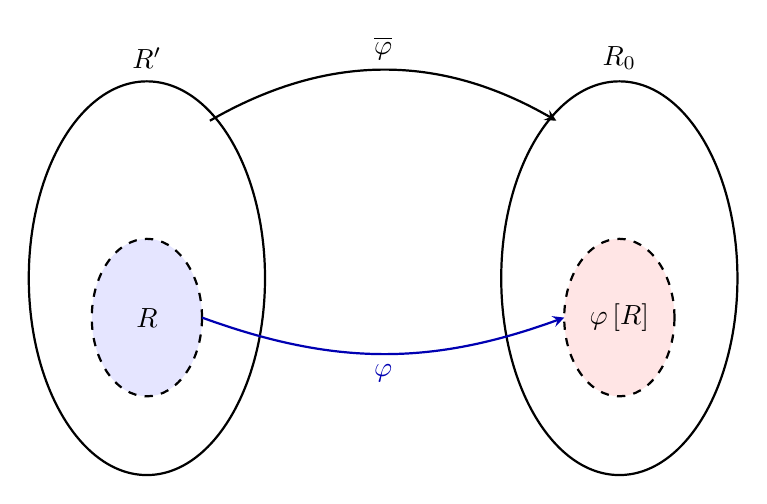
\begin{tikzpicture}[>=stealth, thick]
    % --- DZIEDZINA (X) ---
    % Duża elipsa (cała dziedzina)
    \draw (0,0) ellipse (1.5cm and 2.5cm);
    \node at (0, 2.8) {$R'$};

    % Podzbiór A (mniejsza dziedzina)
    \draw[fill=blue!10, dashed] (0, -0.5) ellipse (0.7cm and 1cm);
    \node (A) at (0, -0.5) {$R$};

    % --- PRZECIWDZIEDZINA (Y) ---
    % Duża elipsa (cała przeciwdziedzina)
    \begin{scope}[xshift=6cm]
        \draw (0,0) ellipse (1.5cm and 2.5cm);
        \node at (0, 2.8) {$R_0$};

        % Podzbiór B (obraz podzbioru A)
        \draw[fill=red!10, dashed] (0, -0.5) ellipse (0.7cm and 1cm);
	\node (B) at (0, -0.5) {$\varphi \left[ R \right]  $};
    \end{scope}

    % --- FUNKCJE (STRZAŁKI) ---
    % Funkcja psi (główna, od góry do góry)
    \draw[->] (0.8, 2) to[bend left=30] node[above] {$\overline{\varphi  }$} (5.2, 2);

    % Funkcja phi (obcięcie, od podzbioru do podzbioru)
    \draw[->, blue!70!black] (0.7, -0.5) to[bend right=20] node[below] {$\varphi$} (5.3, -0.5);

\end{tikzpicture}
\end{center}

	\item $\mathbb{Q} := \mathbb{Z} _{\mathbb{Z} \setminus \{\mathbf{0}\} } = \mathbb{Z}_{0}$
	\item $S\subseteq R$ będzie podzbiorem multiplikatywnym. 
		\[
		\mfaktor{\left( r,s \right) }{E} \mapsto \frac{r}{s} \in R'
		.\] 
\end{enumerate}
Łatwo sprawdzić, że $R_{S}\cong \text{ podpierścień }R'$ złożony z elementów postaci $\frac{a}{b} = ab^{-1}$, dla $a\in R$, $b\in S$. Po takim utożsamieniu $R_{S}$ z podpierścieniem $R'$, możemy przyjąć, że dla $S_1\subseteq S_2$ mamy $R_{\scriptscriptstyle S_1}\underset{\scriptscriptstyle\text{podp}}{\subseteq} R_{\scriptscriptstyle S_2}$.

Na przykład dla $S = 2^{\N} := \{2^{n}: n\in N\} \subseteq \mathbb{Z} $,
mamy 
\[
\mathbb{Z} _{S} := \{\frac{a}{2^{n}}: a \in \mathbb{Z} , n \in \N\} = \mathbb{Z} \left[ \frac{1}{2} \right] \text{ ciało diadyczne}
.\] 

\begin{fact}

	$P$ ideał pierwszy w $R \implies R\setminus P$ jest podzbiorem multiplikatywnym.
\end{fact}
\begin{definition}[Lokalizacja $R$ względem $P$]
	Niech $P$ będzie ideałem pierwszym w $R$. Wtedy: \[
	R_{P} := R_{\scriptscriptstyle R\setminus P}\text{ nazywamy lokalizacją $R$ względem  $P$}
	.\] 
\end{definition} 
\begin{eg}
 $\mathbb{Z} _{(2)} = \mathbb{Z} _{\mathbb{Z} \setminus (2)} = \{\frac{n}{m}\in \mathbb{Q} : n,m\in \mathbb{Z} \text{ oraz }2 \nmid m  \} $
\end{eg} 
\begin{remark}
	
	$\mathbb{Z}_{(2)}\neq \mathbb{Z} _{2^{\N}}$
\end{remark} 
\begin{theorem}
	$P$ jest ideałem pierwszym w $R \implies \left( R_{p} \right)^{\ast} = \{\frac{a}{b}\in R_{p}: a \in R\setminus P\} $
\end{theorem} 
\begin{proof}
	TODO
\end{proof} 
\textbf{Przykłady:}
Niech $K$ będzie ciałem.
\begin{enumerate}[label=\arabic*)]
	\item $\mathbb{Z}_{0} = \mathbb{Q}$
	\item $K\left[ X_1,\ldots,X_{n}  \right] $ oznaczamy przez $K\left( X_1,\ldots,X_{n}  \right) $ 
		i nazywamy \textbf{ciałem funkcji wyższych} ($n$ zmiennych o współczynnikach z $K$ )
	\item $K\left[ \left| X_1,\ldots,X_{n}  \right|  \right] _{0}$ oznaczamy przez $K\left( \left( X_1,\ldots,X_{n}  \right)  \right) $ i nazywamy \textbf{ciałem szeregów Laurenta} ($n$ zmiennych o współczynnikach z $K$.)
\end{enumerate}
\begin{fact}

	$\left(\forall W\in K\left( \left( X \right)  \right)  \right)\left(\exists n\in \N \right)\left(\exists F\in K\left[ \left| X \right|  \right]  \right) W = \frac{F}{X^{n}}   $
\end{fact}
\begin{proof}
	TODO
\end{proof} 
\begin{corollary}
Szeregi Laurenta jednej zmiennej można zapisać w postaci $\sum_{i = -n}^{\infty} a_i x^{i}$ dla $n\in \N$, $a_{i}\in K$.
\end{corollary}
\begin{remark}
	 $K\left( \left( X,Y \right)  \right) \neq \left( K\left( \left( X \right)  \right)  \right) \left( Y \right) $ 
	 Nie ma też zawierania.
\end{remark} 
\begin{context}

	$R$ jest pierścieniem przemiennym z $\mathbf{1} \neq \mathbf{0}$ (niekoniecznie dziedzina)
\end{context}
\begin{definition}[Lokalny]
	$R$ jest \textbf{lokalny}, gdy ma jedyny ideał maksymalny.
\end{definition} 
\begin{theorem}
	Następujące warunki są równoważne:
	\begin{enumerate}[label=\arabic*)]
		\item $R$ jest lokalny,
		\item $\left(\forall a,b \in R\setminus R^{\ast}  \right)\left( a+b \in R\setminus R^{\ast}  \right)  $ 
		\item $R\setminus R^{\ast} \unlhd R$
	\end{enumerate}
\end{theorem} 
\begin{proof}
	TODO
\end{proof} 
\begin{corollary}
	\[
	R \text{ jest lokalny }\iff R \setminus R^{\ast} \text{ jest ideałem} \iff R\setminus R^{\ast} \text{ jest ideałem maksymalnym}
	.\] 
\end{corollary}
\noindent \textbf{Przykłady:} 
\begin{enumerate}[label=\arabic*)]
	\item $K$ jest ciałem $\implies K$ jest lokalny (bo $K\setminus K^{\ast} = \{\mathbf{0}\} \unlhd K $)
	\item $K$ jest ciałem $\implies K\left[ \left| X \right|  \right]^{\ast} = \{\Sigma a_{n} X^{n} \in  K\left[ \left| X \right|  \right] : a_0 \neq \mathbf{0}\} $
	
		\[
		K\left[ \left| X \right|  \right] \setminus K\left[ \left| X \right|  \right] ^{\ast} = \{\Sigma a_{n} X^{n} \in  K\left[ \left| X \right|  \right] : a_0 \neq \mathbf{0}\} = \left( X \right)   
		.\] 
		$(X)$ jest ideałem $\implies K\left[ \left|  X \right|  \right] $ jest lokalny.
\end{enumerate}
\begin{theorem}
	$P \underset{\unlhd }{\text{pierwszy}} R \implies R_{p}$ jest lokalny.
	
\end{theorem} 
\begin{proof}
	TODO
\end{proof} 
